\chapter{Neural Networks: Representation}
\label{chap:neural_net_repr}

Let's start by discussing the motivation for neural networks. We already have seen and coded two powerful machine learning algorithms, so we do we need another? 

\section{Non-linear Hypotheses}
If we have a fairly messy dataset with three terms, $x_1$, $x_2$, and $x_3$, we can classify them using logistic regression, but we'll probably need to introduce polynomial terms to get an accurate classifier. This would give us a hypothesis in the following form:
$$
h_\theta\left(x\right) = g\left(\theta_0, \theta_1 x_1^2 + \theta_2 x_1 x_2 + \theta_3 x_1 x_3 + \theta_4 x_2^2 + \theta_5 x_2 x_3 + \theta_6 x_3^2\right)
$$

Simply by including quadratic terms, we created six features. We can determine this number of features mathematically from combinatorics, and we can model it after sampling with replacement:
\begin{equation}
\text{num. quadratic features } = \binom{n+k-1}{k} = \frac{\left( n + k - 1\right) !}{k! \left(n-1\right)!} = \frac{\left(3 + 2 - 1\right)!}{2! \cdot \left(3-1\right)!} = \frac{4!}{4} = 6
\end{equation}

If we think back to our housing example, and want to perform classification instead of regression using 100 features, that would give us 5050 polynomial terms to include, in addition to the 100 linear terms. We can approximate the growth of the number of new features we get with all quadratic terms with $\mathcal{O}\left(n^2 / 2\right)$. If we wanted to include cubic terms in our hypothesis too, the features would grow asymptotically as $\mathcal{O}\left(n^3\right)$. Since the number of features grows so rapidly, the number of quadratic and cubic features very quickly becomes impractical. 

Consider a collection of $50\times 50$ pixel black-and-white photograph, where we want to determine which photographs are of cars. Then the length of our feature vector is $2500$\footnote{If we were using RGB values, this would be $7500$.}, since we have $2500$ individual pixels. Each features here represents the brightness of the pixel. Now if we want to include quadratic features, we have approximately $2500^2 / 2 = 3,125,000$ features. 

\section{Neurons and the Brain}
Neural networks originated when people thought to build algorithms to mimic how the human brain learns. They were popular in the 1980s, but somewhat fell out of use in the 90s; however, there has been a pretty big surge in neural network use lately due to the massive advances in computer hardware and processing speed. 

While it might seem like the human brain learns different things in different brain regions, there is a hypothesis that the brain only uses a single learning algorithm for all its different functions. This was motivated by an experiment where scientists rewired the optical nerve to the auditory cortex in animals, and the auditory cortex actually learned to see. This was repeated with other areas of the brain as well. The principle behind this is called neuroplasticity.

\section{Model Representation I}
Neural networks were developed to simulate neurons and networks of neurons in the brain. Very simplistically, the neuron takes inputs via the dendrites as electrical inputs (called spikes) and then channels the output via the axon. 

For an artificial neural network, we'll use a very simple model of what a neuron does, we'll model a neuron as a logistic unit. In our model, our inputs are the input features $x_1$, $x_2$, etc. and the output is the result of our hypothesis function. Just like with logistic regression, we have two parameter vectors $\vec{x}$ and $\vec{\theta}$
$$
\vec{x} = \left[\begin{array}{c}x_0 \\ x_1 \\ x_2 \\ x_3 \end{array}\right] ~~\mbox{ \;\;\;\;\;\;\;\;\;\; }~~ \vec{\theta} = \left[\begin{array}{c}\theta_0 \\ \theta_1 \\ \theta_2 \\ \theta_3 \end{array}\right]
$$
where $x_0 = 1$ is the bias term. When representing neural networks, we always have the $\theta_0$ bias term, but we sometimes omit it for notational convenience. Additionally, when representing neural networks, we'll typically use $3$ features, though in reality the number of features is a parameter of the problem. 

$$
\left[\begin{array}{c} x_0 \\ x_1 \\ x_2 \\ x_3 \end{array}\right] \to \left[ {\;\;} \right] \to h_\theta\left(x\right)
$$

We use the same logistic function in the hypothesis as logistic regression. However, in neural networks, it is often called the sigmoid function, or the sigmoid/logistic activation function. 
\begin{equation}
\frac{1}{1 + e^{-\theta^{{}^\intercal} x}}
\end{equation}
We sometimes call the $\theta$ parameters \textbf{weights} for neural networks, as is traditional in the neural network literature, so now we might refer to $\vec{\theta}$ as either parameters or weights. Now, let's look at a very simple model of a neural network. The first layer, $\vec{x}$, is called the \textbf{input layer}. The output of the hypothesis function is called the \textbf{output layer}, which gives the our final value for the hypothesis. In between the input layer and the final layer, there are one or more hidden layers.
\begin{figure}[h] %  figure placement: here, top, bottom, or page
	\centering
	\graphicspath{{./Figures/}} %Use this to import an image from a subfolder.
	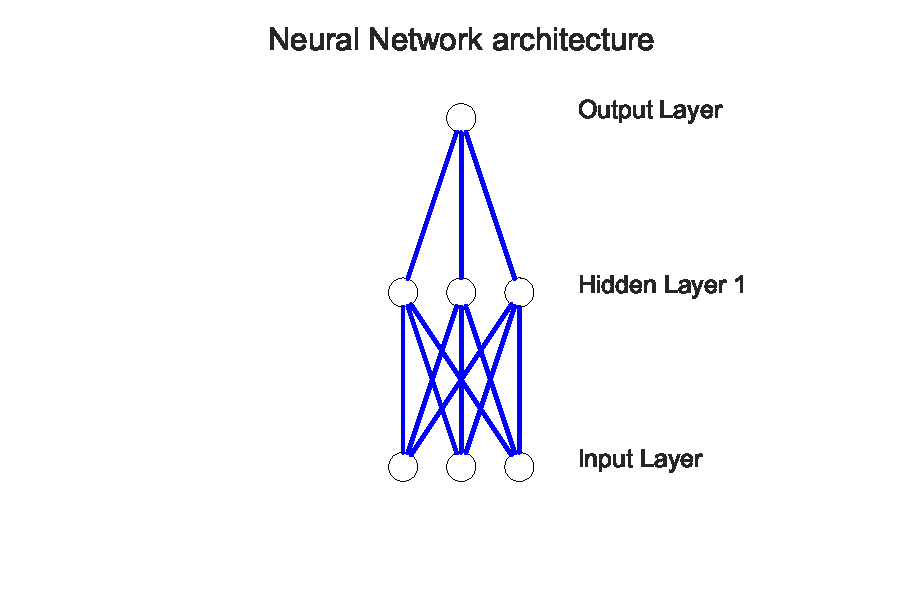
\includegraphics[scale=0.8]{nn_repr_3_layer_neural_netw.pdf} 
	\caption[]{A sample artificial neural network, with three inputs and one hidden layer.}
	\label{nn_repr_3_layer_neural_netw.pdf}
\end{figure}
The hidden layer nodes are labeled $a_1^{(2)}$, $a_2^{(2)}$, etc. and called activation units, where $a_i^{(j)}$ is the activation of unit $i$ in layer $j$. The matrix $\Theta^{(j)}$ is the matrix of weights controlling the function mapping from layer $j$ to layer $j + 1$. Mathematically, we might represent this as
$$
\left[\begin{array}{c} x_0 \\ x_1 \\ x_2 \\ x_3 \end{array}\right] \to \left[\begin{array}{c} a_1^{(2)} \\ a_2^{(2)} \\ a_3^{(2)} \end{array}\right] \to h_\Theta\left(x\right)
$$

Now, let's break out the computations that are represented by this diagram
\begin{subequations}
\begin{align}
a_1^{(2)} &= g\left(	\Theta_{10}^{(1)} x_0 + \Theta_{11}^{(1)} x_1 + \Theta_{12}^{(1)} x_2 + \Theta_{13}^{(1)} x_3   	\right) \\
a_2^{(2)} &= g\left(	\Theta_{20}^{(1)} x_0 + \Theta_{21}^{(1)} x_1 + \Theta_{22}^{(1)} x_2 + \Theta_{23}^{(1)} x_3   	\right) \\
a_3^{(2)} &= g\left(	\Theta_{30}^{(1)} x_0 + \Theta_{31}^{(1)} x_1 + \Theta_{32}^{(1)} x_2 + \Theta_{33}^{(1)} x_3   	\right) \\
h_\Theta\left(x\right) = a_1^{(3)} &= g\left(	\Theta_{10}^{(2)} a_0^{(2)} + \Theta_{11}^{(2)} a_1^{(2)} + \Theta_{12}^{(2)} a_2^{(2)} + \Theta_{13}^{(2)} a_3^{(2)}   	\right) 
\end{align}
\label{chapnnrepr-sectmodelrepr1-definehiddenlayeractivations}
\end{subequations}
This is saying that we compute our activation nodes using a $3\times 4$ matrix or parameters. We apply each row of parameters to our inputs to obtain the value for one activation node. Our hypothesis output is the sigmoid function applied to the sum of the values from the activation nodes, which have been multiplied by yet another parameter matrix, $\Theta^{(2)}$, containing the weights for our second layer of nodes. 

More generally, the dimension of the matrix of weights $\Theta^{(j)}$ is given by the following: if a network has $s_j$ units in layer $j$, and $s_{j+1}$ units in later $j+1$, then $\Theta^{(j)}$ will have dimensions 
\begin{equation}
\| \Theta^{(j)} \| = \left(s_{j+1}\right)\times\left(s_j + 1\right)
\end{equation}
The $+1$ for layer $j$ comes from the bias nodes, $x_0$ and $\Theta_0^{(j)}$, and it's only applied to the input nodes since the output of a layer doesn't include a bias node. 

For example, if layer one has $2$ input nodes and layer two has $4$ activation nodes, then $\Theta^{(1)}$ will be a $4\times 3$ matrix, since $s_j = s_1 = 2$ and $s_{j+1} = s_2 = 4$.

\section{Model Representation II}
Now, we're going to go through the neural network model again, but this time with a vectorized implementation. We begin by defining a new variable $z_k^{(j)}$ that encompasses the parameters inside of our sigmoid function $g$. As such, we can now rewrite equations \ref{chapnnrepr-sectmodelrepr1-definehiddenlayeractivations} as
\begin{align*}
a_1^{(2)} &= g\left(	\Theta_{10}^{(1)} x_0 + \Theta_{11}^{(1)} x_1 + \Theta_{12}^{(1)} x_2 + \Theta_{13}^{(1)} x_3   	\right) & &\implies &  a_1^{(2)} &= g\left(z_1^{(2)}\right) \\
a_2^{(2)} &= g\left(	\Theta_{20}^{(1)} x_0 + \Theta_{21}^{(1)} x_1 + \Theta_{22}^{(1)} x_2 + \Theta_{23}^{(1)} x_3   	\right) & &\implies &  a_2^{(2)} &= g\left(z_1^{(2)}\right) \\
a_3^{(2)} &= g\left(	\Theta_{30}^{(1)} x_0 + \Theta_{31}^{(1)} x_1 + \Theta_{32}^{(1)} x_2 + \Theta_{33}^{(1)} x_3   	\right) & &\implies &  a_3^{(2)} &= g\left(z_1^{(2)}\right)
\end{align*}
So the $z$ values are just a weighted linear combination of the input values $x_0$, $x_1$, etc. going to a particular neuron. In other words, for layer $j=2$ and node $k$, 
\begin{equation}
z_k^{(2)} = \Theta_{k, 0}^{(1)} x_0 + \Theta_{k, 1}^{(1)} x_1 + \cdots + \Theta_{k, n}^{(1)} x_n
\end{equation}
The vector representations of $x$ and $z^{(j)}$ are
$$
x = \left[\begin{array}{c} x_0 \\ x_1 \\ x_2 \\ x_3 \end{array}\right] ~~\mbox{ \;\;\;\;\;\;\;\;\;\; }~~ z^{(j)} = \left[\begin{array}{c} z_1^{(j)} \\ z_2^{(j)} \\ z_3^{(j)} \end{array}\right]
$$
From these vectors, we have $z^{(2)} = \Theta^{(1)} x$ and $a^{(2)} = g\left(z^{(2)}\right)$, where $z^{(2)} \in \mathbb{R}^3$ and $a^{(2)} \in \mathbb{R}^3$. We define $x$ to be $a^{(1)}$, which makes sense because $x$ is our input vector and $a^{(1)}$ implies that we're looking at our first layer, which is the input layer. Then, we can write the general definition for $z$ as
\begin{equation}
z^{(j)} = \Theta^{(j-1)} a^{(j-1)}
\end{equation}
Here, we are multiplying our matrix $\Theta^{(j-1)}$, with dimensions $s_j \times (n+1)$, by our vector $a^{j-1}$, with length $(n+1)$. This yields our vector $z^{(j)}$ with length $s_j$.\footnote{Recall that $s_j$ is the number of activation nodes.} 

From this, we can create a vector of our activation nodes for layer $j$ as 
\begin{equation}
a^{(j)} = g\left(z^{(j)}\right)
\end{equation}
where the sigmoid function $g$ is applied element-wise to $z^{(j)}$. Next, to get our hypothesis, we need to add a bias term to the layer $j=2$, $a_0^{(2)} = 1$. In fact, we can generalize going forward that we will need to add bias terms, and they'll all equal one $a_0^{(j)} = 1$. Now, we have $a^{(2)} \in \mathbb{R}^4$, since we just added the bias term to the previously length-three vector. Now, we can compute 
$$
z^{(3)} = \Theta^{(2)} a^{(2)}
$$
and 
$$
h_\Theta\left(x\right) = a^{(3)} = g\left(z^{(3)}\right)
$$

This process for computing $h_\Theta\left(x\right)$ is called \textbf{forward propagation}, because we start off with the activations of the input units, then forward propagate that to compute the activations of the hidden layer, then again forward propagate that to compute the activations of the output layer. 

Let's step back for a minute. What we're doing here is very similar to logistic regression, though it might not seem like it. Previously, we have the input feed directly into the logistic regression; now instead, we have the nodes from layer $j=2$ (the hidden layer) feeding into the logistic regression. However, those nodes $a_k^{(2)}$ are themselves learned from the input data

We've been specifically talking about the neural network architecture described in Figure \ref{nn_repr_3_layer_neural_netw.pdf}, but there can be other neural network architectures too. Consider the example shown in Figure \ref{nn_repr_4_layer_neural_netw.pdf}.
\begin{figure}[h] %  figure placement: here, top, bottom, or page
	\centering
	\graphicspath{{./Figures/}} %Use this to import an image from a subfolder.
	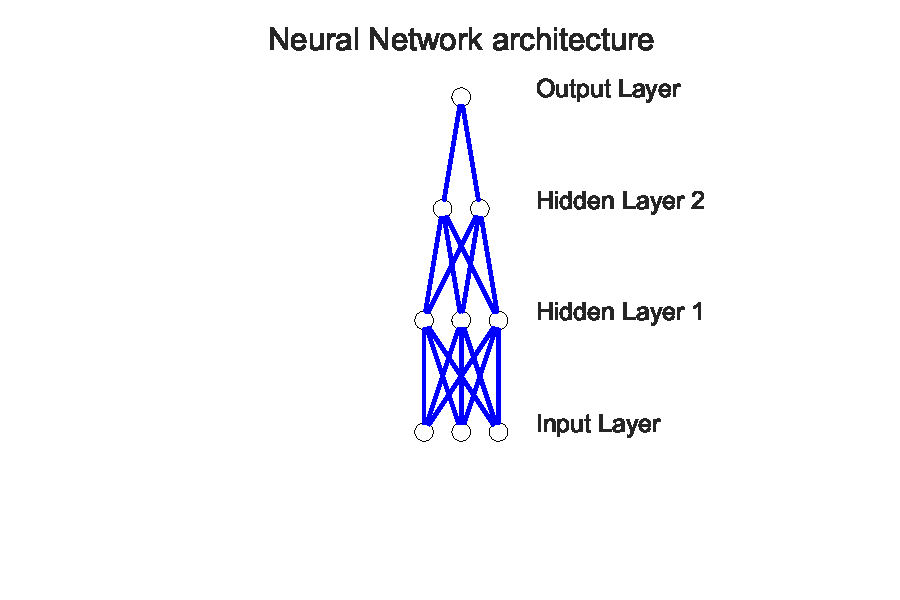
\includegraphics[scale=1]{nn_repr_4_layer_neural_netw.pdf} 
	\caption[]{A sample artificial neural network, with three inputs and two hidden layer.}
	\label{nn_repr_4_layer_neural_netw.pdf}
\end{figure}
Here, we have the same input layer, but there are two hidden layers. The first hidden layer has three hidden units, which are computed as some complex function of the input layer. The second hidden layer can take the first hidden layer's features and compute even more complex features, so the output layer can have very complex features. 


\section{Examples and Intuitions}
Let's say we have inputs $x_1, x_2 \in \{0, 1\}$. In this case, our target label $y = x_1 \text{ AND } x_2$. This is a logical \textit{and}. Can we make a neural network that can recreate this \textit{and} operator? The graph of our function will look something like this
$$
\left[\begin{array}{c} x_0 \\ x_1 \\ x_2 \end{array}\right] \to \left[g\left(z^{(2)}\right)\right] \to h_\Theta\left(z\right)
$$
where $x_0 = 1$ is our bias variable. For this example, let's define our first $\Theta^{(1)}$ matrix as
$$
\Theta^{(1)} = \left[\begin{array}{ccc}\Theta_{1,0}^{(1)} & \Theta_{1,1}^{(1)} & \Theta_{1,2}^{(1)} \end{array}\right] = \left[\begin{array}{ccc}-30 & 20 & 20 \end{array}\right]
$$
This means our hypothesis is given by 
$$
h_\Theta\left(x\right) = g\left(	-30 + 20x_1 + 20x_2	\right)
$$
Let's figure out what our hypothesis evaluates to for different combinations of $x_1$ and $x_2$\footnote{Keep in mind that the sigmoid function evaluates to about $0.99$ for an input of $4.6$, and about $0.01$ for an input value of $-4.6$.}

\begin{center}
\begin{tabular}{c c | r}
$x_1$ & $x_2$ & $h_\Theta\left(x\right)$ \\
\hline
$0$ & $0$ & $g\left(-30\right) \approx 0$ \\
$0$ & $1$ & $g\left(-10\right) \approx 0$ \\
$1$ & $0$ & $g\left(-10\right) \approx 0$ \\
$1$ & $1$ & $g\left(10\right) \approx 1$
\end{tabular}
\end{center}

This is exactly the truth table for the logical \textit{and}, so $h_\Theta\left(x\right) \approx x_1 \text{ AND } x_2$. Using a small neural network, we have just constructed one of the most fundamental operations in computing: the \textit{and} gate. 

\subsection{Building Logical Gates Using Neural Networks}
We are also able to build neural networks to simulate all other logical gates. Let's start with a super-simple example. If we have a single input variable $x_1$, let's use a neural network to build the logical \textit{not} gate. We could do this with 
$$
\Theta^{(1)} = \left[\begin{array}{cc}\Theta_{1,0}^{(1)} & \Theta_{1,1}^{(1)} \end{array}\right] = \left[\begin{array}{cc}10 & -20 \end{array}\right]
$$
giving us a hypothesis of
$$
h_\Theta\left(x\right) = g\left(10 - 20x\right)
$$
If we fill out the table of values for this, we get
\begin{center}
\begin{tabular}{c | r}
$x_1$ & $h_\Theta\left(x\right)$ \\
\hline
$0$ & $g\left(10\right) \approx 1$ \\
$1$ & $g\left(-10\right) \approx 0$
\end{tabular}
\end{center}
As a reminder, here is a truth table for some additional logic gates.
\begin{center}
\begin{tabular}{| c | c | c | c | c | c | c | c |} \hline
\multicolumn{2}{| c |}{\textbf{Input}} & \multicolumn{6}{ c |}{\textbf{Output}} \\ \hline
A & B & A and B & A or B & A nand B & A nor B & A xor B & A xnor B \\ \hline \hline
0 & 0 & 0 & 0 & 1 & 1 & 0 & 1 \\ \hline
0 & 1 & 0 & 1 & 1 & 0 & 1 & 0 \\ \hline
1 & 0 & 0 & 1 & 1 & 0 & 1 & 0 \\ \hline
1 & 1 & 1 & 1 & 0 & 0 & 0 & 1 \\ \hline
\end{tabular}
\end{center}

We can similarly construct $\Theta$ for the \textit{or} gate as
$$
\Theta^{(1)} = \left[\begin{array}{ccc}\Theta_{1,0}^{(1)} & \Theta_{1,1}^{(1)} & \Theta_{1,2}^{(1)} \end{array}\right] = \left[\begin{array}{ccc}-10 & 20 & 20 \end{array}\right]
$$
and $\Theta$ for the \textit{nor} gate as
$$
\Theta^{(1)} = \left[\begin{array}{ccc}\Theta_{1,0}^{(1)} & \Theta_{1,1}^{(1)} & \Theta_{1,2}^{(1)} \end{array}\right] = \left[\begin{array}{ccc}10 & -20 & -20 \end{array}\right]
$$


\subsection{Logical XNOR Gate}
Having defined the \textit{not}, \textit{and}, \textit{or}, and \textit{nor} gates, let's try and build a logical \textit{xnor} gate. We'll start by building a hidden layer with two nodes, one built with the \textit{and} gate and the other with the \textit{nor} gate. Using 
$$
\Theta^{(1)} = \left[\begin{array}{ccc} -30 & 20 & 20 \\ 10 & -20 & -20 \end{array}\right]
$$
we can build $a_1^{(2)}$ from the \textit{and} gate and build $a_2^{(2)}$ from the \textit{or} gate. This gives us the following 
\begin{center}
\begin{tabular}{c c | c c | c}
$x_1$ & $x_2$ & $ a_1^{(2)}$ & $a_2^{(2)}$ & $h_\Theta\left(x\right)$ \\ \hline
0 & 0 & 0 & 1 & {} \\
0 & 1 & 0 & 0 & {} \\
1 & 0 & 0 & 0 & {} \\
1 & 1 & 1 & 0 & {}
\end{tabular}
\end{center}
Now, to finish our \textit{xnor} gate, we can use the $\textit{or}$ gate between our two existing nodes on the second layer. 
$$
\Theta^{(2)} = \left[\begin{array}{ccc} -10 & 20 & 20 \end{array}\right]
$$
Writing this out formally, we find
\begin{align*}
a^{(2)} &= g\left(\Theta^{(1)} x\right) \\
h_\Theta\left(x\right) = a^{(3)} &= g\left(\Theta^{(2)} a^{(2)}\right)
\end{align*}
Filling in the rest of our table, we find we've built the \textit{xnor} gate!
\begin{center}
\begin{tabular}{c c | c c | c}
$x_1$ & $x_2$ & $ a_1^{(2)}$ & $a_2^{(2)}$ & $h_\Theta\left(x\right)$ \\ \hline
0 & 0 & 0 & 1 & 1 \\
0 & 1 & 0 & 0 & 0 \\
1 & 0 & 0 & 0 & 0 \\
1 & 1 & 1 & 0 & 1
\end{tabular}
\end{center}


\section{Multiclass Classification}
Similar to logistic regression, we can do multiclass classification with neural networks, and the way we do it is essentially an extension of the one-vs-all method. Let's say we have a computer vision example, where we're trying to classify an image into a pedestrian, a car, a motorcycle, or a truck. We would do this buy building a neural network with an output of four numbers, meaning the output $h_\Theta$ will actually be a $4$-vector. In our example, when we have a pedestrian or car, we'd want our output to be
$$
\text{(pedestrian) } h_\Theta\left(x\right) \approx \left[\begin{array}{c} 1 \\ 0 \\ 0 \\ 0 \end{array}\right] ~~\mbox{ \;\;\;\;\;\;\;\;\;\; }~~ \text{(car)} h_\Theta\left(x\right) \approx \left[\begin{array}{c} 0 \\ 1 \\ 0 \\ 0 \end{array}\right]
$$
Our training set will look similar
$$
\left(x^{(1)}, y^{(1)}\right), \left(x^{(2)}, y^{(2)}\right), \left(x^{(3)}, y^{(3)}\right), \cdots, \left(x^{(m)}, y^{(m)}\right)
$$
but instead of representing $y \in \{1, 2, 3, 4\}$, we'll represent $y^{(i)}$ as one of the following:
$$
y^{(i)} \in \left\{	 \left[\begin{array}{c} 1 \\ 0 \\ 0 \\ 0 \end{array}\right],  	\left[\begin{array}{c} 0 \\ 1 \\ 0 \\ 0 \end{array}\right],	 
			\left[\begin{array}{c} 0 \\ 0 \\ 1 \\ 0 \end{array}\right], 	 \left[\begin{array}{c} 0 \\ 0 \\ 0 \\ 1 \end{array}\right]		\right\}
$$
where both $h_\Theta\left(x\right)$ and $\vec{y}$ will be in $\mathbb{R}^4$. 

Let's write this out a bit. Sticking with the image classification problem with four output classes, our artificial neural network can be represented by
$$
\left[\begin{array}{c} x_0 \\ x_1 \\  x_2 \\ x_3 \\ \vdots \\ x_n\end{array}\right] \to
\left[\begin{array}{c} a_0^{(2)} \\ a_1^{(2)} \\ a_2^{(2)} \\ a_3^{(2)} \\ \vdots \end{array}\right] \to 
\left[\begin{array}{c} a_0^{(3)} \\ a_1^{(3)} \\ a_2^{(3)} \\ a_3^{(3)} \\ \vdots \end{array}\right] \to 
\left[\begin{array}{c} h_\Theta\left(x\right)_1 \\ h_\Theta\left(x\right)_2 \\ h_\Theta\left(x\right)_3 \\ h_\Theta\left(x\right)_1 \end{array}\right]
$$
The final hidden layer of nodes, when multiplied by its $\Theta$ matrix, will result in another vector, on which we can apply the sigmoid function $g$ to get a vector of hypothesis values, which will be (asymptotically) equal to one of the four $y^{(i)}$ vectors.  

























